
\chapter{N-ary Tree}
\label{cha:n-ary-tree}

If a tree is a rooted tree in which each node has no more than \argument{N} children, it is called \keyword{N-ary tree}.


Here is an example of 3-ary tree:
\begin{figure}[H]
  \centering
  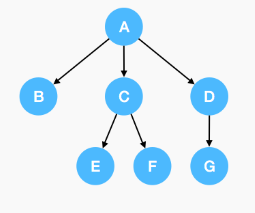
\includegraphics[width=0.5\textwidth]{n-ary-tree}
  \caption{N-ary tree}
  \label{fig:n-ary-tree}
\end{figure}

\keyword{Trie} (Chapter \ref{cha:trie}) is one of the most frequently used N-ary trees.

\section{Travesal}
\label{sec:travesal}


A binary tree can be traversed in preorder, inorder, postorder or level-order.
Among these traversal methods, preorder, postorder and level-order traversal are suitable to be extended to an \keyword{N-ary tree}.


\section{Examples}
\label{sec:examples-5}

Here are some examples on \href{https://github.com/mingmingli916/algorithms/tree/main/n_ary_tree}{Github}.



%%% Local Variables:
%%% mode: latex
%%% TeX-master: "algorithms"
%%% End:
